%%%%%%%%%%%%%%%%%%%%%%%%%%%%%%%%%%%%%%%%%%%%%%%%%%%%%%%%%%%%%%%%%%%%%%
%\title{Project Report}
%
%%% Preamble
\documentclass[paper=a4, fontsize=11pt]{scrartcl}
\usepackage[T1]{fontenc}
\usepackage{fourier}
\usepackage{geometry}
\geometry{margin=1in}
\usepackage{wrapfig}
\usepackage{xcolor}
\usepackage{listings}

\lstdefinestyle{base}{
  language=Python,
  emptylines=1,
  breaklines=true,
  basicstyle=\fontsize{9}{13}\selectfont\ttfamily,
  moredelim=**[is][\color{red}]{@}{@},
}

\usepackage[english]{babel}	
% English language/hyphenation
% GRAPHICS
\usepackage{placeins} 
\usepackage{flafter}  
\usepackage{graphicx} % advanced figure inclusion
\usepackage{float} % specifying table/figure locations, i.e. [ht!]
\usepackage{wrapfig}

\usepackage[small, bf]{caption} 
\captionsetup{format=plain, justification=raggedright,singlelinecheck=false}%change scriptsize of graphic captions
\usepackage{subfig}
\usepackage[protrusion=true,expansion=true]{microtype}	
\usepackage{amsmath,amsfonts,amsthm} % Math packages	

\usepackage{adjustbox}
\usepackage{longtable} % For long tables that span multiple pages
\newcommand{\sym}[1]{\rlap{#1}}% For symbols like *** in tables
\usepackage{tabularx} %  advanced table features
\newcolumntype{L}[1]{>{\raggedright\arraybackslash}p{#1}}
\newcolumntype{C}[1]{>{\centering\arraybackslash}p{#1}}
\newcolumntype{R}[1]{>{\raggedleft\arraybackslash}p{#1}}
\usepackage{relsize} % precise adjustment of font size,

\usepackage{booktabs}
\usepackage{multirow}
\usepackage{upquote}


%%% Custom sectioning
\usepackage{sectsty}
\allsectionsfont{\centering \normalfont\scshape}


%%% Custom headers/footers (fancyhdr package)
\usepackage{fancyhdr}
\pagestyle{fancyplain}
\fancyhead{}											% No page header
\fancyfoot[L]{}											% Empty 
\fancyfoot[C]{}											% Empty
\fancyfoot[R]{\thepage}									% Pagenumbering
\renewcommand{\headrulewidth}{0pt}			% Remove header underlines
\renewcommand{\footrulewidth}{0pt}				% Remove footer underlines
\setlength{\headheight}{13.6pt}


%%% Equation and float numbering
\numberwithin{equation}{section}		% Equationnumbering: section.eq#
\numberwithin{figure}{section}			% Figurenumbering: section.fig#
\numberwithin{table}{section}				% Tablenumbering: section.tab#

%\newcommand{\sectionA}{\renewcommand{\thesection}{\arabic{section}A}\section}
%\newcommand{\sectionB}{\edef\thesection{\arabic{section}B}\addtocounter{section}{-1}\section}


%%% Maketitle metadata
\pagestyle{fancy}
\fancyhf{}
\rhead{David Munoz Tord}
\lhead{Trends in Computational Neuroscience ---Mini-Project 2}
\rfoot{\thepage}


 %Title
\usepackage{titlesec} %customization of titles
\titleformat{\section}{\large\bfseries}{\thesection}{1em}{}
%\titleformat*{\subsection}{\large\bfseries}
\titleformat{\subsection}    
   {\normalfont\bfseries\itshape}{\thesubsection}{1em}{}
\renewcommand{\thesubsection}{\thesection.\alph{subsection}}

%%% Begin document
\begin{document}
\section{Behavioral Modeling}
\subsection{Model Fitting}


\begin{figure}[!hbt]
\begin{center}
 \makebox[\textwidth]{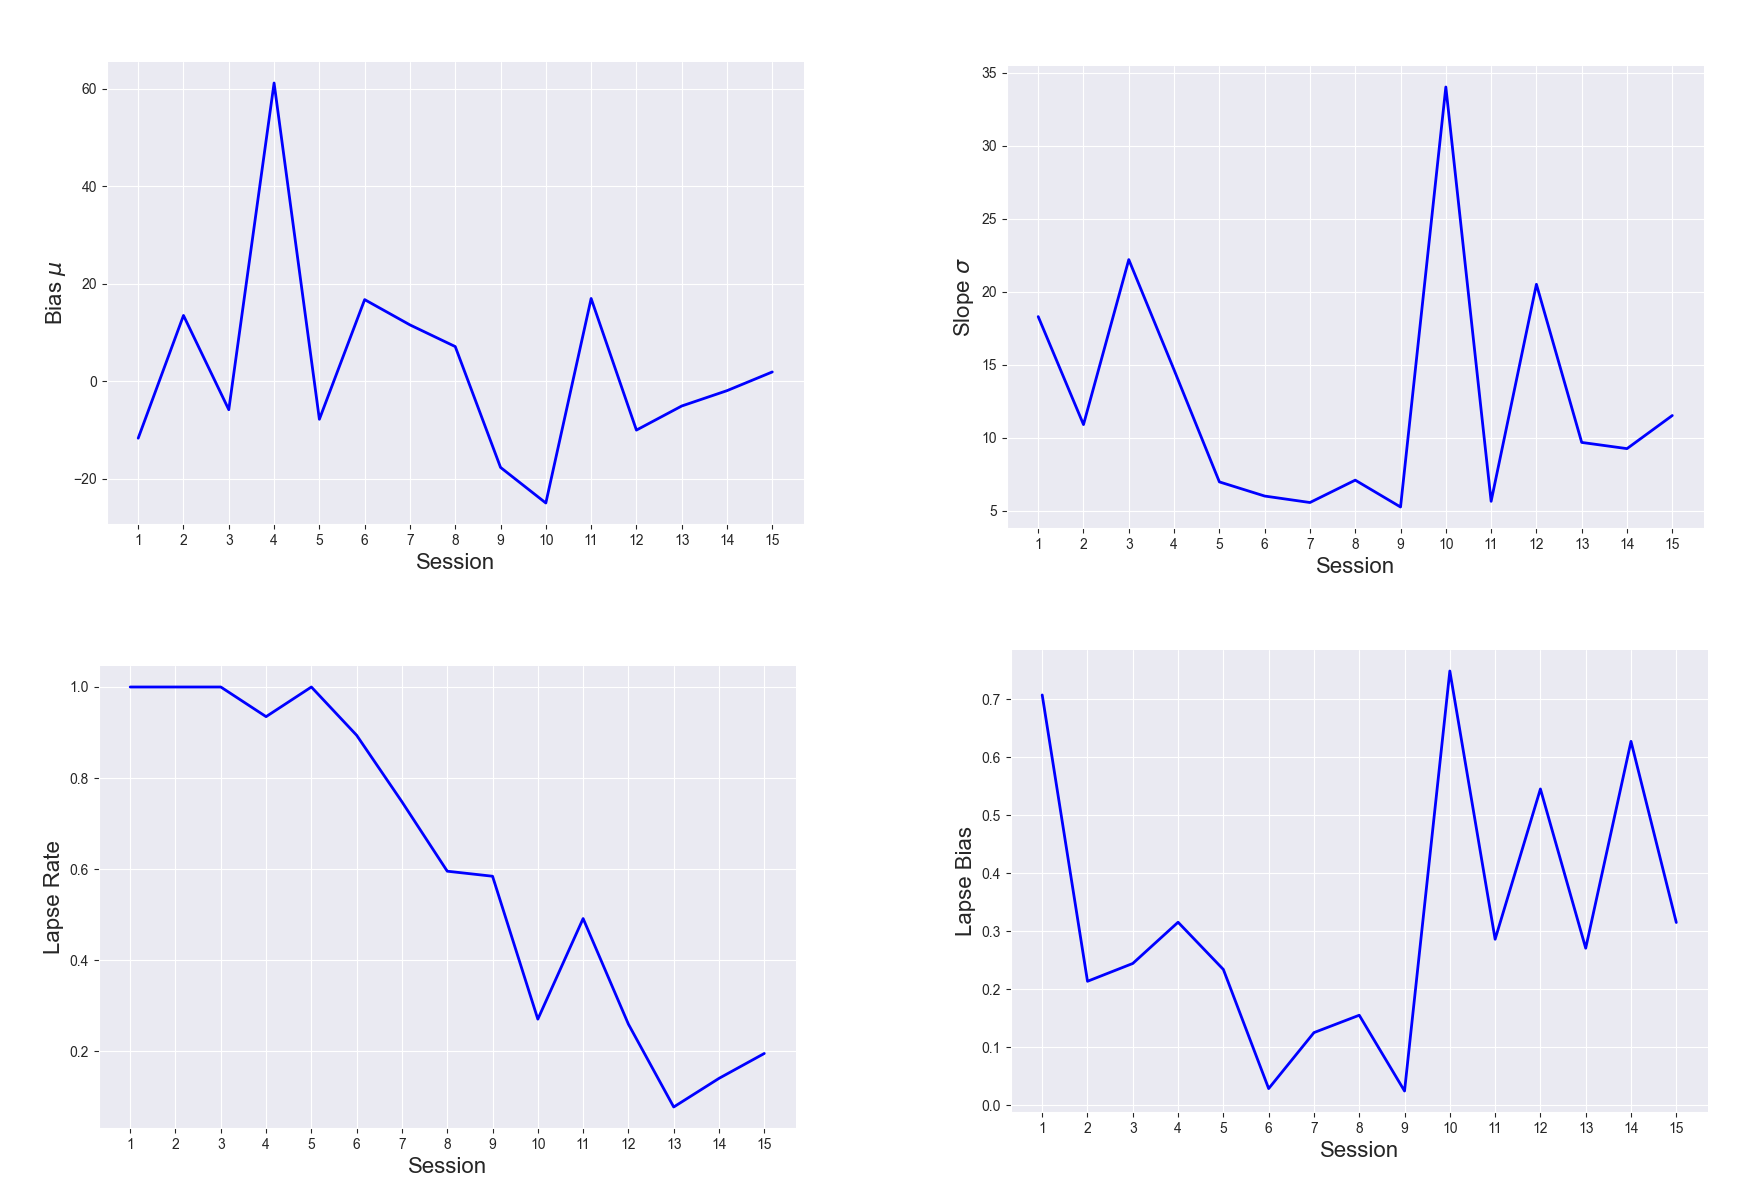
\includegraphics[width=13cm]{full.png}}
\end{center}
\caption{Model parameters (bias, slope/threshold, lapse rate, lapse bias) using maximum-likelihood estimation for a basic psychometric model as a function of training sessions of mouse KS014.}
\label{fig:param}
\end{figure}
We can see on Figure \ref{fig:param} that while the bias parameter (upper right) fluctuates up and above zero for the first sessions (1-7), it starts to steadily tend to zero on the last sessions (12-15) which would represent no preferred bias. Globally, we see a consistent \textquotesingle drift\textquotesingle\ across parameters around the 10th session, this is likely due to the change in the number of contrast conditions in the paradigm. We can observe that paradigm change by looking at the slope parameter (upper left) where the discrimination threshold drastically increase in the 10th session.  The lapse rate parameter (lower roght) is especially interesting because it linearly decrease throughout the training session span, this would likely indicate that the mouse is paying more attention to the task it is asked to perform and act less \textquotesingle randomly\textquotesingle\ when trained. Similarly to the mean bias, the lapse bias seems to converge towards 0.5 which would represent no preferred lapse bias (lower left).





\subsection{Model Selection}
%\begin{figure}[!hbt]
%\begin{center}
 %\makebox[\textwidth]{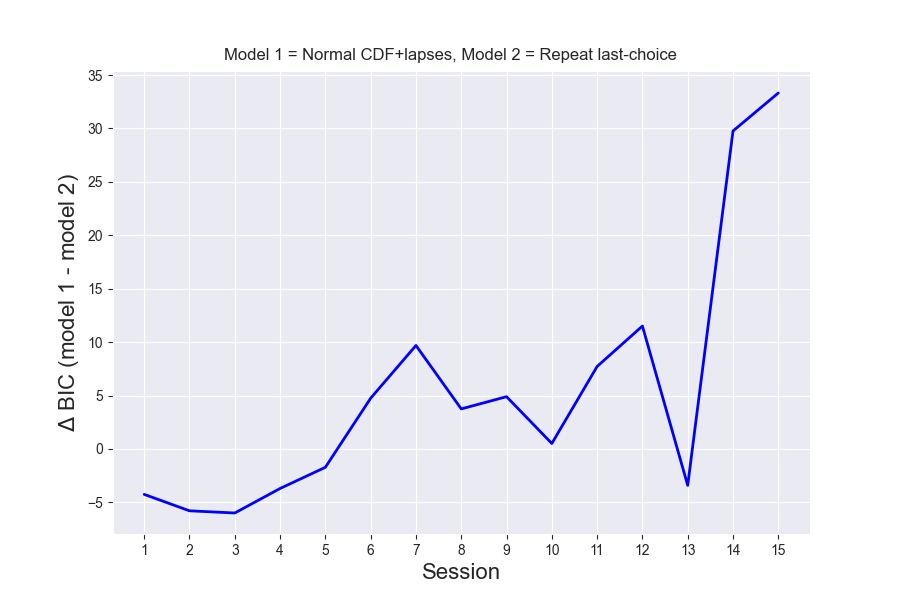
\includegraphics[width=10
% cm]{BIC.png}}
%\end{center}
%\caption{Model comparison metric as a function of training sessions of mouse KS014. Both models parameters where estimated via a maximum-likelihood. Model 1 consist in a basic psychometric function model (normal CDF+lapses) with 4 parameters (bias, slope/threshold, lapse rate, lapse bias), whereas Model 2 consists in the Model 1 with an added 5th parameter (repeat-last) to account for the probability of the auto-correlation of the decision process with the previous trial. Here is represented the difference between the two models' penalized-likelihood criteria ($\Delta$ BIC). A positive value shows stronger evidence for the Model 2 relatively to Model 1.}
%\label{fig:selec}
%\end{wrapfigure}
%\end{figure}

\begin{wrapfigure}{r}{0.5\linewidth}
\vspace{-80pt}
  \begin{center}
    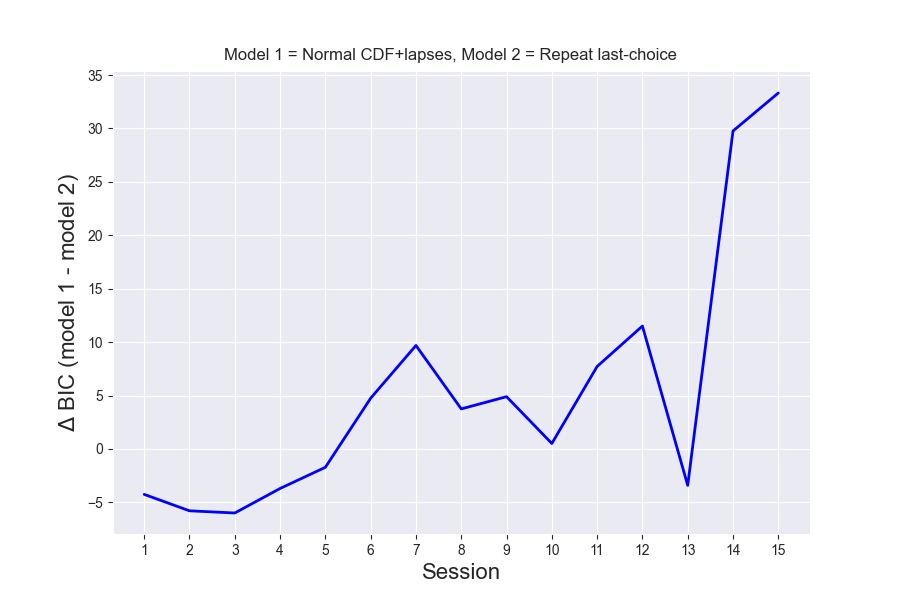
\includegraphics[width=\linewidth]{BIC.png}
  \end{center}
  \vspace{-20pt}
\caption{Model comparison metric as a function of training sessions of mouse KS014. Model 1 consist in a basic psychometric function model with 4 parameters, whereas Model 2 consists in the Model 1 with an added 5th parameter (repeat-last) to account for the probability of the auto-correlation of the decision process with the previous trial. A positive $\Delta$ BIC shows stronger evidence for the Model 2 relatively to Model 1.}
\label{fig:selec}
\end{wrapfigure}

As we can observe from Figure \ref{fig:selec}, the model comparisons metric ($\Delta$ BIC) tends to favor the simplest model on the first 3 sessions but the tendency change from the 5th session towards the last-choice dependent model and peak in the very last sessions. This likely indicates that the adding of a 5th parameter to account for the probability of the response to be the same as the preceding trial (auto-correlation) is only helpful to explain the behavioral data when the the mouse has fully learned to perform the task.



\FloatBarrier

\section{Advanced Model Fitting}
\subsection{Time-Varying Psychometric Model}
\begin{figure}[!hbt]
\begin{center}
 \makebox[\textwidth]{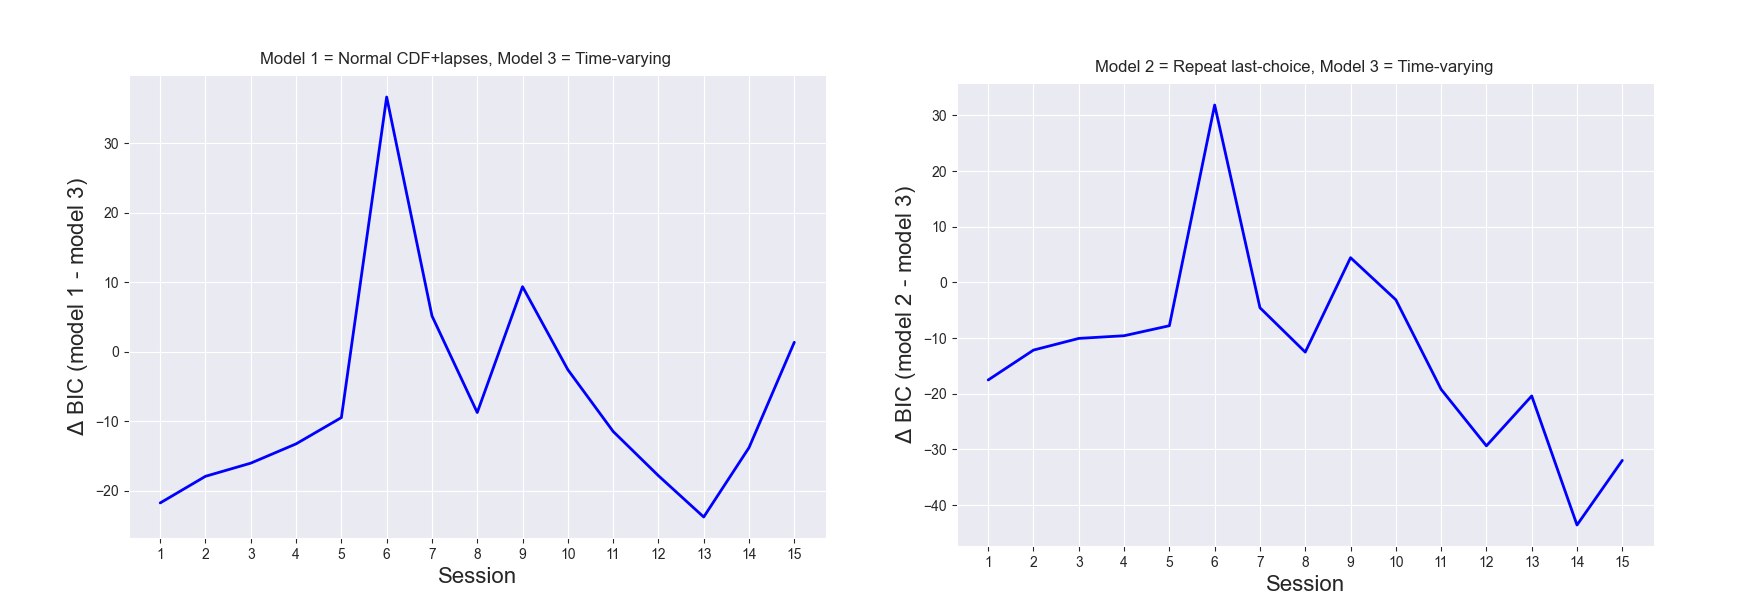
\includegraphics[width=15 cm]{both.png}}
\end{center}
\caption{The difference between the two models ($\Delta$ BIC). A positive value shows stronger evidence for the Model 3 relatively to Model 1.}
\label{fig:time}
\end{figure}




I wasn't particularly inspired and couldn't think of a new model to implement so I just used the already implemented time-varying model except that I rewrited it using vectorization instead of for loops to compute the trial by trial parameters. This made the computing of the 15 sessions 120 times faster. This model (Model 3) consists in 8 parameters and allows to fit them for each trial. As we can see from Figure \ref{fig:time}, Model 3 doesn't really seem to be better than Model 1 according to the $\Delta$ BIC (left). Similar results are obtained when comparing Model 3 to Model 2 (right). This doesn't hold however for session 6 and 10 (even more when looking at AIC that doesn't penalize parameters as much as BIC). This could reflect increased trial-by-trial variability in those session. Indeed, session 6 was done after a \textquotesingle break \textquotesingle and sessions 10 introduced a new condition for the first time.

\begin{lstlisting}[style=base]
def psychofun_vec(theta,stim): """Psychometric function vectorized"""
    @mu = theta[:,0]@           # bias
    @sigma = theta[:,1]@        # slope
    @lapse = theta[:,2]@         # lapse rate
    @lapse_bias = theta[:,3]@    # lapse bias}
    p_right = norm.cdf(stim,loc=mu,scale=sigma)    
    p_right = lapse*lapse_bias + (1-lapse)*p_right # Adding lapses
    return p_right

def psychofun_timevarying_loglike_vec(theta,df):"""Log-likelihood for time-varying model"""
    s_vec = np.array(df['signed_contrast']) # Stimulus values
    r_vec = np.array(df['response_choice'])  # Responses
    Ntrials = len(s_vec)
    mu = np.linspace(theta[0],theta[4],Ntrials)
    sigma = np.linspace(theta[1],theta[5],Ntrials)
    lapseR = np.linspace(theta[2],theta[6],Ntrials)
    lapseB = np.linspace(theta[3],theta[7],Ntrials)
    @ThetaMat = np.transpose(np.asarray([mu,sigma,lapseR,lapseB]))@ 
    @p_right = psychofun_vec(ThetaMat,s_vec)@
    loglike = np.sum(np.log(p_right[r_vec == 1])) + np.sum(np.log(1 - p_right[r_vec == -1]))
    return loglike
\end{lstlisting}

\end{document}